\section{VECSEL Chips}\label{sec:vecsel}

The basic structure of a VECSEl gain chip is shown in \cref{fig:vecDes}. The main feature of the structure are as follows: 

\begin{figure}[ht]
    \centering
    \includegraphics[width=.8\linewidth]{images/VECSEL_structure.png}
    \caption{}
    \label{fig:vecDes}
\end{figure}

\begin{itemize}
    \item Heat spreader: The heat spreader role is in dissipating the heat generated during the operation of the VECSEL chip to a Peltier-stabilized copper heat-sink.
    \item Pump \& laser  DBR: The purpose of the two bottom mirrors is to reflect the laser light and the pump light. Two advantages: firstly, because of higher absorption, there is a higher optical-to-optical efficiency due to the two passes through the active region, and secondly, there is less absorption in the mirror and in the heat sink, which results also in a higher efficiency and a higher maximum output power. The high reflectivity for two wavelengths is realized by using a superlattice Bragg mirror
    \item Active region: The purpose of the active region is the conversion of the pump light into the laser light. The gain medium in the active region is often composed of quantum wells or quantum dots.
    \item Anti-reflection coating: The antireflection section is optimized to reduce the otherwise large reflection from the air/GaAs interface
\end{itemize}

Below the three different structure of the Vecsel chips used in this work.  SEE ETH MAIL

%A distributed Bragg reflector (DBR) for the pump wavelength (808 nm) reflects the unabsorbed pump light, reducing heat deposition in the structure and increasing efficiency.
The DBR for the laser wavelength acts as a flat cavity mirror.


\subsection*{Hybrid chip, SV165}

\begin{wrapfigure}{r}{.5\textwidth}
    \centering
    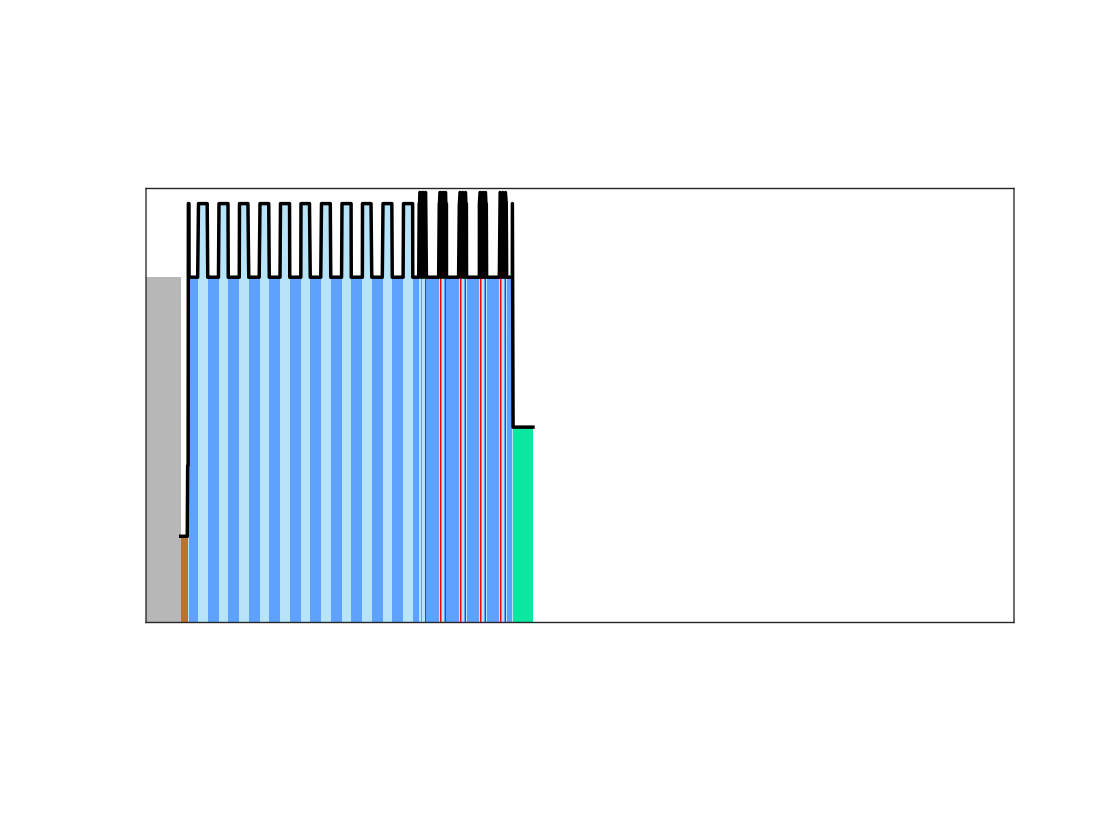
\includegraphics[width=.98\textwidth]{images/1SV165.lay.png}
    \caption{}
    \label{fig:sv165}
\end{wrapfigure}

This was achieved with a backside-cooled, InGaSb-based VECSEL using a hybrid metal-semiconductor Bragg reflector. We demonstrate the fabrication of such a hybrid metal-semiconductor mirror by combining a copper mirror with 10.5 AlAs0.08Sb0.92/GaSb distributed Bragg reflector (DBR) pairs. Together with a thin 20nm SiO2 diffusion barrier we reach >99.9\% reflectivity at 2 um. This allows for a thinner gain chip design compared to the standard DBR requiring 19.5 layer pairs. The structure thickness was reduced from 7.5 um to 4.7 um lowering the thermal resistance of the device from (2.79+-0.16)KW-1 to (2.12+-0.19)KW-1


\subsection*{No pump DBR chip, SV166}

\begin{wrapfigure}{r}{.5\textwidth}
    \centering
    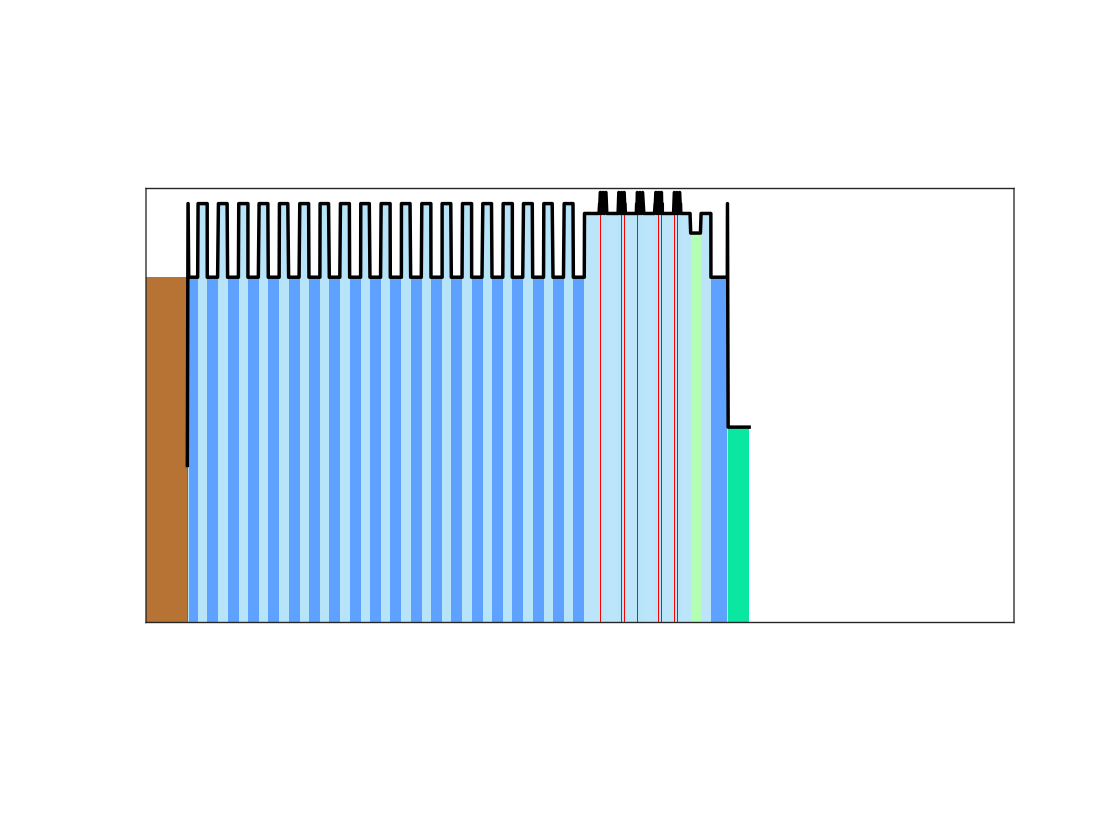
\includegraphics[width=.98\textwidth]{images/1SV166.lay.png}
    \caption{}
    \label{fig:sv166}
\end{wrapfigure}

This was achieved with a backside-cooled, InGaSb-based VECSEL using a hybrid metal-semiconductor Bragg reflector. We demonstrate the fabrication of such a hybrid metal-semiconductor mirror by combining a copper mirror with 10.5 AlAs0.08Sb0.92/GaSb distributed Bragg reflector (DBR) pairs. Together with a thin 20nm SiO2 diffusion barrier we reach >99.9\% reflectivity at 2 um. This allows for a thinner gain chip design compared to the standard DBR requiring 19.5 layer pairs. The structure thickness was reduced from 7.5 um to 4.7 um lowering the thermal resistance of the device from (2.79+-0.16)KW-1 to (2.12+-0.19)KW-1


\subsection*{Pump DBR chip, SV167}

\begin{wrapfigure}{r}{.5\textwidth}
    \centering
    \includegraphics[width=.98\textwidth]{images/1SV167B.lay.png}
    \caption{}
    \label{fig:sv167}
\end{wrapfigure}

This was achieved with a backside-cooled, InGaSb-based VECSEL using a hybrid metal-semiconductor Bragg reflector. We demonstrate the fabrication of such a hybrid metal-semiconductor mirror by combining a copper mirror with 10.5 AlAs0.08Sb0.92/GaSb distributed Bragg reflector (DBR) pairs. Together with a thin 20nm SiO2 diffusion barrier we reach >99.9\% reflectivity at 2 um. This allows for a thinner gain chip design compared to the standard DBR requiring 19.5 layer pairs. The structure thickness was reduced from 7.5 um to 4.7 um lowering the thermal resistance of the device from (2.79+-0.16)KW-1 to (2.12+-0.19)KW-1



\subsection{VECSEL model}